
\chapter*{Solitons: Korteweg-deVries Equation}
\addcontentsline{toc}{chapter}{Solitons: Korteweg-deVries Equation}
	\marginpar{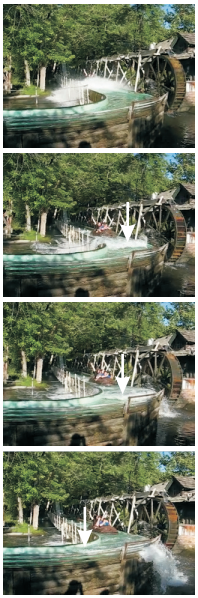
\includegraphics[width=\marginparwidth]{fig1201}\captionof{figure}{The log flume ride at Lagoon produces a solitary wave (marked by arrows in the frames above). The leading edge of the soliton is where the water begins to spill over the side of the trough.}\label{fig:48}}
At the Lagoon amusement park in Utah, there is a water ride called the Log Flume. It is a standard, old-fashioned water ride where people sit in a 6-seater boat shaped like a log which slowly travels along a fiberglass trough through some scenery, then is pulled up a ramp to an upper level. The slow ascent is followed by a rapid slide down into the trough below, which splashes the passengers a bit, after which the log slowly makes its way back to the loading area. But you can see something remarkable happen as you wait your turn to ride if you watch what happens to the water in the trough when the log splashes down. A large water wave is pushed ahead of the log, as you might expect. But instead of gradually dying away, as you might think a single pulse should in a dispersive system like surface waves on water, the pulse lives on and on. It rounds the corner ahead of the log that created it, enters the area where logs are waiting to be loaded, pushes each log up and down in turn, then heads out into the scenery beyond, still maintaining its shape.

This odd wave is called a \rq\rq soliton\lq\lq, or \rq\rq "solitary wave\lq\lq, and it is an interesting feature of non-linear dynamics that has been widely studied in the last 30 years, or so. The simplest mathematical equation which produces a soliton is the KortewegdeVries equation
\begin{equation}\label{eq:1201}
\frac{\partial y}{\partial t}+y \frac{\partial y}{\partial x}+\alpha \frac{\partial^{3} y}{\partial x^{3}}=0
\end{equation}
which describes surface waves in shallow water. In the first two terms of this
equation you can see the convective behavior we studied in Lab 10, but the last
term, with its rather odd third derivative, is something new. We will be studying
this equation in this laboratory.

\section*{Numerical solution for the Korteweg-deVries equation}
\addcontentsline{toc}{section}{Numerical solution for the Korteweg-deVries equation}
We will begin our study of the Korteweg-deVries equation by using Crank-Nicolson to finite difference it on a grid so that we can explore its behavior by numerical experimentation. The first step is to define a grid, and since we want to be able to see the waves travel for a long time we will copy the trough at Lagoon and make our computing region be a closed loop. We can do this by choosing an interval from $x=0$ to $x=L$, as usual, but then we will make the system be periodic by declaring that $x=0$ and $x=L$ are actually the same point, as would be the case in a circular trough. We will subdivide this region into $N$ subintervals and let $h=L / N$ and $x_{j}=(j-1) h$, so that the grid is cell-edge. Normally such a cell-edge grid would have $N+1$ points, but ours doesn't because the last point $(j=N)$ is just a repeat of the first point: $x_{N}=x_{0}$, because our system is periodic.\\
We now do the usual Crank-Nicolson differencing, where we evaluate each term in the equation at time level $n+1 / 2$. The last term in Eq. \eqref{eq:1201} has a third derivative, so we\rq ll need a reasonable approximation for the third derivative. Suppose you have function values $f(x-3 h / 2), f(x-h / 2), f(x+h / 2)$, and $f(x+$ $3 h / 2)$. A good way to do this is to write down four Taylor's series up to the fifth derivative for the function at these four points and then solve this system of four equations to find expressions for $f(x), f^{\prime}(x), f^{\prime \prime}(x)$, and $f^{\prime \prime \prime}(x)$. This procedure yields the approximate formula

\begin{equation}\label{eq:1202}
f^{\prime \prime \prime}(x) \approx \frac{f(x+3 h / 2)-3 f(x+h / 2)+3 f(x-h / 2)-f(x-3 h / 2)}{h^{3}}
\end{equation}

along with an error term on the order of $h^{2}$. When we time average Eq. \eqref{eq:1202}, we find

\begin{equation}\label{eq:1203}
\alpha \frac{\partial^{3} y}{\partial x^{3}}=\frac{\alpha}{2 h^{3}}\left(y_{j+2}^{n+1}-3 y_{j+1}^{n+1}+3 y_{j}^{n+1}-y_{j-1}^{n+1}+y_{j+2}^{n}-3 y_{j+1}^{n}+3 y_{j}^{n}-y_{j-1}^{n}\right)
\end{equation}
	\marginpar{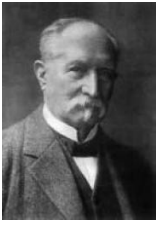
\includegraphics[width=\marginparwidth]{korteweg}\\ Diederik Korteweg (1848-1941, Dutch)}
		\marginpar{\includegraphics[width=\marginparwidth]{vries}\\ Gustav de Vries (1866-1934, Dutch) Diederik Korteweg was Gustav\rq s dissertation advisor.}

Look closely at Eq. \eqref{eq:1203} and also at Eq. \eqref{eq:1202} to convince yourself that they are not centered on a grid point, but at spatial location $j+1 / 2$. The use of this third derivative formula thus adds a new twist to the usual Crank-Nicolson differencing: we will evaluate each term in the equation not only at time level $n+1 / 2$, but also at spatial location $j+1 / 2$ (at the center of each subinterval) so that the first and third derivative terms are both properly centered. This means that we will be using a cell-edge grid, but that the spatial finite differences will be cell centered.
With this wrinkle in mind, we can write the first term in Eq. \eqref{eq:1201} at time level $n+1 / 2$ and space location $j+1 / 2$ as

\begin{equation}\label{eq:1204}
\frac{\partial y}{\partial t}=\frac{1}{2 \tau}\left(y_{j}^{n+1}+y_{j+1}^{n+1}-y_{j}^{n}-y_{j+1}^{n}\right)
\end{equation}

Now we have have to decide what to do about the nonlinear convection term $y \partial y / \partial x$. We will assume that the leading $y$ is known somehow by designating it as $\bar{y}$ and decide later how to properly estimate its value. Recalling again that we need to evaluate at time level $n+1 / 2$ and space location $j+1 / 2$, the non-linear term becomes

\begin{equation}\label{eq:1205}
y \frac{\partial y}{\partial x}=\frac{\bar{y}_{j+1}+\bar{y}_{j}}{4 h}\left(y_{j+1}^{n+1}-y_{j}^{n+1}+y_{j+1}^{n}-y_{j}^{n}\right)
\end{equation}

For now, we\rq ve ignored the problem that the derivative in Eq. \eqref{eq:1205} is centered in time at $n+1 / 2$ while the $\bar{y}$ term isn't. We\rq ll have to deal with this issue later.
Each of these approximations in Eqs. \eqref{eq:1203}-\eqref{eq:1205} is now substituted into Eq. \eqref{eq:1201}, the $y^{n+1}$ terms are gathered on the left side of the equation and the $y^{n}$ terms are gathered on the right, and then the coefficients of the matrices $\mathbf{A}$ and $\mathbf{B}$ are read off to put the equation in the form
\begin{equation}\label{eq:1206}
\mathbf{A} y^{n+1}=\mathbf{B} y^{n}
\end{equation}
in the usual Crank-Nicolson way. If we denote the four nonzero elements of A
and B like this:
\begin{equation}\label{eq:1207}
\begin{array}{ll}
A_{j, j-1}=a_{--} & A_{j, j}=a_{-} \\
A_{j, j+1}=a_{+} & A_{j, j+2}=a_{++} \\
B_{j, j-1}=b_{--} & B_{j, j}=b_{-} \\
B_{j, j+1}=b_{+} & B_{j, j+2}=b_{++}
\end{array}
\end{equation}

then the matrix coefficients turn out to be

\begin{equation}\label{eq:1208}
\begin{array}{ll}
a_{--}=-\frac{\alpha}{2 h^{3}} & a_{-}=\frac{1}{2 \tau}+\frac{3 \alpha}{2 h^{3}}-\frac{\left(\bar{y}_{-}+\bar{y}_{+}\right)}{4 h} \\
a_{+}=\frac{1}{2 \tau}-\frac{3 \alpha}{2 h^{3}}+\frac{\left(\bar{y}_{-}+\bar{y}_{+}\right)}{4 h} & a_{++}=\frac{\alpha}{2 h^{3}} \\
b_{--}=\frac{\alpha}{2 h^{3}} & b_{-}=\frac{1}{2 \tau}-\frac{3 \alpha}{2 h^{3}}+\frac{\left(\bar{y}_{-}+\bar{y}_{+}\right)}{4 h} \\
b_{+}=\frac{1}{2 \tau}+\frac{3 \alpha}{2 h^{3}}-\frac{\left(\bar{y}_{-}+\bar{y}_{+}\right)}{4 h} & b_{++}=-\frac{\alpha}{2 h^{3}}
\end{array}
\end{equation}
where $y_{-}=y_{j}$ and where $y_{+}=y_{j+1}$, the grid points on the left and the right of the $j+1 / 2$ spatial location (where we are centering).

\begin{problem}\label{P12.1}
Derive the formulas in Eq. \eqref{eq:1208} for the $a$ and $b$ coefficients using the finite-difference approximations to the three terms in the Korteweg-deVries equation given in Eqs. \eqref{eq:1203}-\eqref{eq:1205}.
\end{problem}
Now that the coefficients of $\mathbf{A}$ and $\mathbf{B}$ are determined we need to worry about how to load them so that the system will be periodic. For instance, in the first row of $A$ the entry $A_{1,1}$ is $a_{-}$, but $a_{--}$should be loaded to the left of this entry, which might seem to be outside of the matrix. But it really isn\rq t, because the system is periodic, so the point to the left of $j=1$ (which is also the point $j=(N+1)$ ) is the point $j-1=N$. The same thing happens in the last two rows of the matrices as well, where the subscripts $+$ and $++$ try to reach outside the matrix on the right. So correcting for these periodic effects makes the matrices $\mathbf{A}$ and $\mathbf{B}$ look like this:
\begin{equation}\label{eq:1209}
\begin{aligned}
\mathbf{A} &=\left[\begin{array}{cccccccc}
a_{-} & a_{+} & a_{++} & 0 & 0 & \ldots & 0 & a_{--} \\
a_{--} & a_{-} & a_{+} & a_{++} & 0 & \ldots & 0 & 0 \\
0 & a_{--} & a_{-} & a_{+} & a_{++} & \cdots & 0 & 0 \\
. & . & . & . & \ldots & . & . & . \\
0 & \ldots & 0 & 0 & a_{--} & a_{-} & a_{+} & a_{++} \\
a_{++} & 0 & \ldots & 0 & 0 & a_{--} & a_{-} & a_{+} \\
a_{+} & a_{++} & 0 & 0 & \ldots & 0 & a_{--} & a_{-}
\end{array}\right] \\
\mathbf{B} &=\left[\begin{array}{cccccccc}
b_{-} & b_{+} & b_{++} & 0 & 0 & \ldots & 0 & b_{--} \\
b_{--} & b_{-} & b_{+} & b_{++} & 0 & \ldots & 0 & 0 \\
0 & b_{--} & b_{-} & b_{+} & b_{++} & \cdots & 0 & 0 \\
. & . & . & . & \ldots & . & . & . \\
0 & \ldots & 0 & 0 & b_{--} & b_{-} & b_{+} & b_{++} \\
b_{++} & 0 & \ldots & 0 & 0 & b_{--} & b_{-} & b_{+} \\
b_{+} & b_{++} & 0 & 0 & \cdots & 0 & b_{--} & b_{-}
\end{array}\right]
\end{aligned}
\end{equation}

\begin{problem}\label{P12.2}Discuss these matrices with a TA and convince the TA that this structure correctly models a periodic system (it may help to think about the computing grid as a circle with $x_{0}=x_{N}$.)
\end{problem}
\begin{equation}\label{eq:1210}
\tilde{v}=v^{n}
\end{equation}


\begin{equation}\label{eq:1211}
v^{p}=\mathbf{A}\left(v^{n}\right)^{-1}\left[\mathbf{B}\left(v^{n}\right) v^{n}\right]
\end{equation}

\begin{equation}\label{eq:1212}
v^{*}=\frac{v^{p}+v^{n}}{2}
\end{equation}
\begin{equation}\label{eq:1213}
v^{n+1}=\mathbf{A}\left(v^{*}\right)^{-1}\left[\mathbf{B}\left(v^{*}\right) v^{n}\right]
\end{equation}
All right, that\rq s it. You may have the feeling by now that this will all be a little tricky to code, and it is. We would rather have you spend the rest of the time in this lab doing physics instead of coding, so below (and on the course web site) you will find a copy of a Python program $\mathrm{kdv}$. py that implements this algorithm. You and your lab partner should carefully study the script to see how each step of the algorithm described above is implemented, then work through the problems listed below by running the script and making appropriate changes to it.

\section*{Solitons}
\addcontentsline{toc}{section}{Solitons}

\begin{problem}\label{P12.3}
	\marginpar{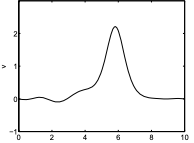
\includegraphics[width=\marginparwidth]{fig1202}\captionof{figure}{A Gaussian pulse after 1 second of propagation by the Korteweg-deVries equation (Problem 12.3)}\label{fig:49}}

\begin{enumerate}[label=(\alph*)]
\item Run kdv . py with $\alpha=0.1, y_{\max }=2, \tau=0.5, t_{\text {final }}=100$, and iskip $=1$. After a while you should see garbage on the screen. This is to convince you that you shouldn't choose the time step to be too large.
\item Now run (a) again, but with $\tau=0.1$, then yet again with $\tau=0.02$. Use $t_{\text {final }}=10$ for both runs and skip big enough that you can see the pulse moving on the screen. You should see the initial pulse taking off to the right, but leaving some bumpy stuff behind it as it goes. The trailing bumps don\rq t move as fast as the big main pulse, so it laps them and runs over them as it comes in again from the left side, but it still mostly maintains its shape. This pulse is a soliton. You should find that there is no point in choosing a very small time step; $\tau=0.1$ does pretty well.

\end{enumerate}
\end{problem}
The standard \rq\rq lore \lq\lq in the field of solitons is that the moving bump you saw in problem $12.3$ is produced by a competition between the wave spreading caused by the third derivative in the Korteweg-deVries equation and the wave steepening caused by the $y \partial y / \partial x$ term. Let\rq s run $\mathrm{kdv}$. py in such a way that we can see the effect of each of these terms separately.


\begin{problem}\label{P12.4}
\begin{enumerate}[label=(\alph*)]
\item Dispersion (wave-spreading) dominates: Run $\mathrm{kdv}$. py with $\alpha=0.1$, $y_{\max }=0.001, \tau=0.1$, and $t_{\text {final }}=10$. The small amplitude makes the nonlinear convection term $y \partial y / \partial x$ be so small that it doesn't matter; only the third derivative term matters. You should see the pulse fall apart into random pulses. This spreading is similar to what you saw when you solved Schrödinger's equation. Different wavelengths have different phase velocities, so the different parts of the spatial Fourier spectrum of the initial pulse get out of phase with each other as time progresses.
\item Non-linear wave-steepening dominates: Run $\mathrm{kdv}$. py with $\alpha=0.01$, $y_{\max }=2, \tau=0.01$, and $t_{\text {final }}=10$. (If your solution develops short wavelength wiggles this is an invitation to use a smaller time step. The problem is that the predictor-correction algorithm we used on the nonlinear term is not stable enough, so we have a Courant condition in this problem.)
Now it is the dispersion term that is small and we can see the effect of the non-linear convection term. Where $y$ is large the convection is rapid, but out in front where $y$ is small the convection is slower. This allows the fast peak to catch up with the slow front end, causing wave steepening. (An effect just like this causes ocean waves to steepen and then break at the beach.)
\end{enumerate}
\end{problem}
The large pulse that is born out of our initial Gaussian makes it seem like
there ought to be a single pulse that the system wants to find. This is, in fact the
case. It was discovered that the following pulse shape is an exact solution of the
Korteweg-deVries equation:

	\marginpar{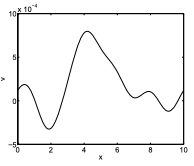
\includegraphics[width=\marginparwidth]{fig1203}\captionof{figure}{ Dispersion dominates (Problem 12.4(a).): after 3 seconds of time.}\label{fig:50}}
	\marginpar{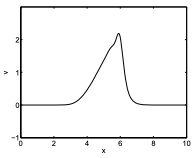
\includegraphics[width=\marginparwidth]{fig1204}\captionof{figure}{ Steepening dominates (Problem $12.4(b) .$ ): after $0.5$ seconds of time.}\label{fig:51}}

\begin{equation}\label{eq:1214}
y(x, t)=\frac{12 k^{2} \alpha}{\cosh ^{2}\left(k\left(x-x_{0}-4 \alpha k^{2} t\right)\right)}
\end{equation}
where $x_0$ is the center of the pulse at time $t = 0$.

\begin{problem}\label{P12.5}
\begin{enumerate}[label=(\alph*)]
\item Use Mathematica to show that this expression does indeed satisfy the
Korteweg-deVries equation
\item Now replace the Gaussian initial condition in $\mathrm{kdv}$. py with this pulse shape, using $k=1.1, x_{0}=L / 2$, and adjusting $\alpha$ so that the height of the initial pulse is exactly equal to 2, so that it matches the Gaussian pulse you ran in 12.3. You should find that this time the pulse does not leave trailing pulses behind, but that it moves without changing shape. It is a perfect soliton.
\item The formula at the beginning of this problem predicts that the speed of the pulse should be 
\begin{equation}\label{eq:1215}
c_{\text {soliton }}=4 \alpha k^{2}
\end{equation}
Verify by numerical experimentation that your soliton moves at this speed. To do this, you can just track the position of the maximum value (the NumPy function ar gmax can help you do this).
\end{enumerate}
\end{problem}
\begin{problem}\label{P12.6}
One of the most interesting things about solitons is how two of them interact with each other. When we did the wave equation earlier you saw that left and right moving pulses passed right through each other. This happens because the wave equation is linear, so that the sum of two solutions is also a solution. The Korteweg-deVries equation is nonlinear, so simple superposition can't happen. Nevertheless, two soliton pulses do interact with each other in a surprisingly simple way.

To see what happens keep $\alpha=0.1$, but modify your code from $12.5$ so that you have a soliton pulse with $k=1.5$ centered at $x=3 L / 4$ and another soliton pulse with $k=2$ centered at $x=L / 4$. Run for about 20 seconds and watch how they interact when the fast large amplitude pulse in the back catches up with the slower small amplitude pulse in the front. Is it correct to say that they pass through each other? If not, can you think of another qualitative way to describe their interaction?
\end{problem}
\begin{lstlisting}
import matplotlib.pyplot as plt
import numpy as np
import scipy.linalg as la

# Physical constants
alpha = 0.1

# Make the grid
N = 500
L = 10
h = L/N
x = np.linspace(h/2,L-h/2,N)

# Initial Gaussian centered on the computing region
ymax = 2
y = ymax * np.exp(-(x-.5*L)**2)

# Time range
tau = 0.1
tfinal = 100
t = np.arange(0,tfinal,tau)

# Initialize the parts of the A and B matrices that
# do not depend on ybar and load them into At and Bt.
# Make them be sparse so the code will run fast.
At = np.zeros((N,N))
Bt = np.zeros((N,N))

# Function to wrap the column index
def jwrap(j):
	if (j < 0):
		return j + N
	if (j >= N):
		return j - N
	return j
# load the matrices with the terms that don't depend on ybar
h3 = h**3
for j in range(N):
	At[j,jwrap(j-1)] =-0.5*alpha/h3
	At[j,j] = 0.5/tau + 1.5*alpha/h3
	At[j,jwrap(j+1)] = 0.5/tau - 1.5*alpha/h3
	At[j,jwrap(j+2)] = 0.5*alpha/h3

	Bt[j,jwrap(j-1)] = 0.5*alpha/h3
	Bt[j,j] = 0.5/tau - 1.5*alpha/h3
	Bt[j,jwrap(j+1)] = 0.5/tau + 1.5*alpha/h3
	Bt[j,jwrap(j+2)] =-0.5*alpha/h3
	
	
plt.figure(1)
skip = 10
for n in range(len(t)):
	# Predictor step
	A = np.copy(At)
	B = np.copy(Bt)
	
	# load ybar, then add its terms to A and B
	ybar = np.copy(y)
	for j in range(N):
		tmp = 0.25*(ybar[jwrap(j+1)] + ybar[j])/h
		A[j,j] = A[j,j] - tmp
		A[j,jwrap(j+1)] = A[j,jwrap(j+1)] + tmp
		B[j,j] = B[j,j] + tmp
		B[j,jwrap(j+1)] = B[j,jwrap(j+1)] - tmp
		
		# do the predictor solve
		r = B@y
		yp = la.solve(A,r)
		
		# corrector step
		A = np.copy(At)
		B = np.copy(Bt)
		
		# average current and predicted y values to correct ybar
		ybar=.5*(y+yp)
		for j in range(N):
			tmp = 0.25*(ybar[jwrap(j+1)] + ybar[j])/h
			A[j,j] = A[j,j] - tmp
			A[j,jwrap(j+1)] = A[j,jwrap(j+1)] + tmp
			B[j,j] = B[j,j] + tmp
			B[j,jwrap(j+1)] = B[j,jwrap(j+1)] - tmp
			
		# do the final corrected solve
		r = B@y
		y = la.solve(A,r)
		
		if (n % skip == 0):
			plt.clf()
			plt.plot(x,y)
			plt.xlabel('x')
			plt.ylabel('y')
			plt.title('time={:1.3f}'.format(t[n]))
			plt.ylim(0,3)
			plt.pause(.1)
\end{lstlisting}
